\documentclass[graybox]{svmult}
%\usepackage{mathptmx}       % selects Times Roman as basic font
%\usepackage{helvet}         % selects Helvetica as sans-serif font
%\usepackage{courier}        % selects Courier as typewriter font
%\usepackage{type1cm}        % activate if the above 3 fonts are
                            % not available on your system
%
%\usepackage{makeidx}         % allows index generation
\usepackage{graphicx}        % standard LaTeX graphics tool
                             % when including figure files
%\usepackage{multicol}        % used for the two-column index
%\usepackage[bottom]{footmisc}% places footnotes at page bottom
\usepackage{amsfonts, amssymb}

%\makeindex             % used for the subject index
                       % please use the style svind.ist with
                       % your makeindex program

%%%%%%%%%%%%%%%%%%%%%%%%%%%%%%%%%%%%%%%%%%%%%%%%%%%%%%%%%%%%%%%%%%%%%%%%%%%%%%%%%%%%%%%%%

\newcommand{\dom}{\mathop{\rm dom}}
\renewcommand{\Im}{\mathop{\rm Im}}
\newcommand{\supp}{\mathop{\rm supp}}
\newcommand{\sgn}{\mathop{\rm sgn}}
\newcommand{\rank}{\mathop{\rm rank}}
\renewcommand{\kappa}{\varkappa}
\newcommand{\rmi}{{\rm i}}
\newcommand{\Real}{\mathbb R}
\newcommand{\Cmpl}{\mathbb C}
\newcommand{\eps}{\varepsilon}
\newcommand{\en}{{\nu,\eps}}
\newcommand{\cI}{\mathcal{I}}
\newcommand{\cF}{\mathcal{F}}
\newcommand{\mv}[1]{\langle #1 \rangle_0}
\newcommand{\fm}[1]{\langle #1 \rangle_1}
\newcommand{\fpr}[1]{{#1}^{(-1)}}
\newcommand{\spr}[1]{{#1}^{(-2)}}
\newcommand{\ra}{\rangle}
\newcommand{\la}{\langle}
\newcommand{\fra}{\mathfrak{a}}

% MATH -----------------------------------------------------------
\newcommand{\norm}[1]{\left\Vert#1\right\Vert}
\newcommand{\abs}[1]{\left\vert#1\right\vert}
\newcommand{\set}[1]{\left\{#1\right\}}
\newcommand{\To}{\longrightarrow}
\newcommand{\BX}{\mathbf{B}(X)}
\newcommand{\A}{\mathcal{A}}
% ----------------------------------------------------------------


\newcommand{\mg}[1]{{\color{magenta}{#1}}}
\newcommand{\rd}[1]{{\color{red}{#1}}}
\renewcommand{\emph}[1]{{\textit{#1}}}
\renewcommand{\phi}{\varphi}
\newcommand\rmd{\mathrm{d}}
\newcommand\rme{\mathrm{e}}
\newcommand\rmR{\mathrm{R}}
\renewcommand{\leq}{\leqslant}
\renewcommand{\geq}{\geqslant}
\newcommand{\myIm}{\mathop{\rm Im}}
\newcommand{\myRe}{\mathop{\rm Re}}
\newcommand{\sign}{\mathop{\rm sign}}
\newcommand{\ess}{\mathop{\rm ess}}
\newcommand{\bl}[1]{{\color{blue}{#1}}}
\newcommand{\oB}[1]{\langle{#1},g\rangle\hskip1pt f+\langle{#1},f\rangle\hskip1pt g}
\newcommand\nep{\textstyle\frac n\eps}
\newcommand\te{\left(\frac t\eps\right)}
\newcommand\se{\left(\frac s\eps\right)}
\newcommand\pfg{p}
\newcommand\hy{\hat{y}_\eps}
\newcommand{\eqref}[1]{(\ref{#1})}
\newcommand{\pte}{\partial_t}
\newcommand{\pts}{\partial_s}

\begin{document}

\title*{Schr\"{o}dinger operators with}
%\titlerunning{Short Title}
\author{Yuriy Golovaty}
%\authorrunning{Short Title}
\institute{Yuriy Golovaty \at Ivan Franko National University of Lviv,
1, Universytetska str., Lviv, 79000, Ukraine \\ \email{yuriy.golovaty@lnu.edu.ua}}

\maketitle

\abstract*{Each chapter should be preceded by an abstract (10--15 lines long) that summarizes the content. The abstract will appear \textit{online} at \url{www.SpringerLink.com} and be available with unrestricted access.}

\abstract{Each chapter should be preceded by an abstract (10--15 lines long) that summarizes the content. The abstract will appear \textit{online} at \url{www.SpringerLink.com} and be available with unrestricted access. }



%%%%%%%%%%%%%%%%%%%%%%%%%%%%%%%%%%%%%%%%%%%%%%%%%%%%%%%%%%%%%%%%%%%%%%%%%%
% Introduction
%%%%%%%%%%%%%%%%%%%%%%%%%%%%%%%%%%%%%%%%%%%%%%%%%%%%%%%%%%%%%%%%%%%%%%%%%%

\section{Introduction  }
\label{Sec:Introduction}



%%%%%%%%%%%%%%%%%%%%%%%%%%%%%%%%%%%%%%%%%%%%%%%%%%%%%%%%%%%%%%%%%%%%%%%%%%
% Statement of Problem and Main Results
%%%%%%%%%%%%%%%%%%%%%%%%%%%%%%%%%%%%%%%%%%%%%%%%%%%%%%%%%%%%%%%%%%%%%%%%%%

\section{Statement of Problem and Main Results}
\label{Sec:Statment}

Let us consider the family of operators
\begin{equation}\label{OprHe}
H_\eps=-\Delta +W(x)+V_\eps(x).
\end{equation}
Suppose that the unperturbed operator $H_0=-\Delta +W$ is self-adjoint in $L^2(\Real^2)$ with a domain $\dom H_0$. In addition, we assume that the potential $W$ belongs to $L^\infty_{loc}(\Real^2)$.

Let $\gamma$ be a  closed $C^3$-curve without self-intersection
points. We will denote by $\omega_\eps$ the $\eps$-neighborhood of $\gamma$, i.e., the union of all open balls with radius $\eps$ and center on~$\gamma$.  Suppose that potentials $V_\eps$ have compact supports that lie in $\omega_\eps$ and  the supports  shrink to curve $\gamma$ as $\eps\to 0$.


To specify  the dependence of $V_\eps$ on  small parameter $\eps$ we introduce  curvilinear coordinates coordinates in $\omega_\eps$.
Let $S$ be the circle of the same length as the length of $\gamma$.
We will parameterize $\gamma$ by points of the circle.
Let $\alpha\colon\; S\to \Real^2$ be the unit-speed $C^3$-parametrization of $\gamma$ with the natural parameter $s\in S$.
Also  $\nu=(-\dot{\alpha}_2, \dot{\alpha}_1)$ is the unit normal on $\gamma$, because  $\dot{\alpha}_1^2+\dot{\alpha}_2^2=1$.
We define the local coordinates $(s,n)$ in $\omega_\eps$ by
\begin{equation}\label{LocalTr}
    x=\alpha(s)+n\nu(s), \qquad (s,n)\in Q_\eps=S\times (-\eps, \eps).
\end{equation}
The coordinate $n$ is the signed distance from a point $x$ to $\gamma$.
Therefore  $\omega_\eps$ is diffeomorphic to cylinder $Q_\eps$ for $\eps$ small enough. There is no loss of generality in assuming the diffeomorphism exists for $\eps\in (0,1)$.

\begin{figure}[b]
\centering
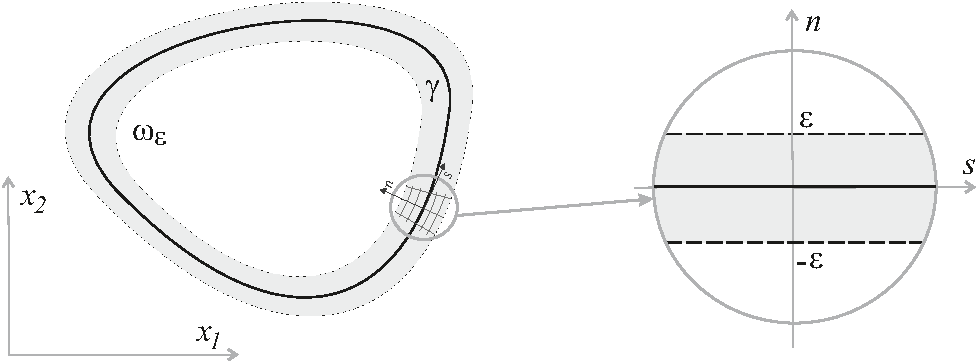
\includegraphics[scale=.6]{LocalCoords}
\caption{Curvilinear coordinates in the $\eps$-neighbourhood of $\gamma$.}
\label{FigLocalCoords}
\end{figure}


We suppose that the localized potentials have the following structure
\begin{equation}\label{Veps}
V_\eps(\alpha(s)+n\nu(s))=\eps^{-2}\,V\left(\eps^{-1}n\right)
+\eps^{-1}\,U\left(s,\eps^{-1}n\right),
\end{equation}
where $V$ and $U$ are measurable bounded functions such that $\supp V\subset (-1,1)$ and $\supp U\subset Q_1$. The key assumption is that $V$ does not depend on  $s$.
The family of potentials $V_\eps$ generally diverges in the space of distributions $\mathcal{D}(\Real^2)$.
As we will show later in Propositin~\ref{PropVepsConverg},
the  potentials converge only if $V$ is a zero mean function, namely
$$
   V_\eps(x)\to a \partial_\nu\delta_\gamma+b\delta_\gamma\quad \mbox{ as \ }\eps\to 0,
$$
where $\delta_\gamma$ is Dirac's delta function supported on $\gamma$, i.e., $\langle\delta_\gamma, \phi\rangle=\int_\gamma \phi \,d \gamma$,  and $a$, $b$ are some functions on $\gamma$.

We now introduce some notation. The plane is divided into two domains by close curve $\gamma$.  We suppose that $\Real^2\setminus\gamma=\Omega_{in}\cup\Omega_{out}$, where domain $\Omega_{out}$ is unbounded. Let us introduce the subspace $\mathcal{V}\subset L_2(\Real^2)$ as follows.
We say that $v$ belongs to $\mathcal{V}$ if $v|_{\Omega_-}\in W_2^2(\Omega_{in})$ and there exist a function $h$ belonging to $\dom H_0$ such that $v=h$ in $\Omega_{out}$. Of course, $v|_{\Omega_{out}}\in W_{2, loc}^2(\Omega_{out})$.

Let $\mathcal{V}_0$ be the subspaces of $L_2(\Omega_{out})$
obtained by the restriction of all elements of $\mathcal{V}$ to $\Omega_{out}$.   We introduce two operators
\begin{eqnarray}\nonumber
&&\mathcal{D}_1= -\Delta+W, \qquad \dom \mathcal{D}_1=\{v\in \mathcal{V}_0\colon\; v=0 \;\,\mbox{on } \gamma\},\\\nonumber
&&\mathcal{D}_2= -\Delta+W, \qquad \dom \mathcal{D}_2=\{v\in W_2^2(\Omega_{in})\colon\; v=0 \;\,\mbox{on } \gamma\}.
\end{eqnarray}


We also denote by $\gamma_t=\{x\in\Real^2\colon\; x=\alpha(s)+t\nu(s), \; s\in S\}$ the closed curve that is obtained from $\gamma$ by flowing for ``time'' $t$ along the normal vector field. Then the boundary of $\omega_\eps$ consists of two curves $\gamma_{-\eps}$ and $\gamma_{\eps}$. For each $v\in \mathcal{V}$ there exist two one-side traces on $\gamma$, namely
$$
  v_-=\lim_{\eps\to 0}v|_{\gamma_{-\eps}}, \qquad
v_+=\lim_{\eps\to 0}v|_{\gamma_{\eps}}.
$$






We say that the Schr\"odinger operator~$-\frac{d^2}{d t^2}+V$ in $L_2(\Real)$ possesses a \emph{half-bound state} (or \emph{zero-energy resonance}) if there exists a non trivial solution~$h$ of the equation $-h'' +Vh= 0$ that is bounded on the whole line.  In this case, we will simply say that potential $V$ possesses a half-bound state.
Such a solution~$h$ is  unique up to a scalar factor and has nonzero limits
$$
  h(-\infty)=\lim\limits_{t\to-\infty}h(t), \qquad
  h(+\infty)=\lim\limits_{t\to+\infty}h(t)
$$
at both the infinities. We set
\begin{equation}\label{Theta}
  \theta=\frac{h(+\infty)}{h(-\infty)}.
\end{equation}



Our main result reads as follows.


\begin{theorem}\label{MainThrm}
For each measurable bounded function $V$ and $U$ of compact support, the family of operators
$
 H_\eps=-\Delta +W+V_\eps,
$
where the perturbation $V_\eps$ is given by \eqref{Veps},
converges as $\eps\to 0$ in the strong resolvent sense.

If potential $V$ possesses a zero-energy resonance with a half-bound state $h$, then operators $H_\eps$ converge to  operator $\mathcal{H}$
defined by
$
\mathcal{H} v=-\Delta v+Wv
$
on functions $v\in \mathcal{V}$  obeying the interface conditions
\begin{equation}\label{ConnectedCond}
 u_+-\theta u_-=0,\quad  \theta\partial_\nu u_+-\partial_\nu u_-
=\left(\textstyle\frac{1}{2 }(\theta^2-1)\kappa+\mu\right) u_-
\end{equation}
on curve $\gamma$. Here  $\theta$ is given by  \eqref{Theta},  $\kappa$ is the signed curvature of $\gamma$, and
 \begin{equation}\label{Mu}
  \mu=\frac{1}{h^2(-\infty)} \int_{-1}^1 U(\,\cdot\,,t)h^2(t)\, dt.
 \end{equation}


Otherwise, if potential $V$ has no zero-energy resonance, then operators $H_\eps$ converge to the direct sum $\mathcal{D}_1\oplus\mathcal{D}_2$ of two unperturbed operators $-\Delta +W$ in $\Omega_{in}$ and $\Omega_{out}$ respectively subject to the Dirichlet boundary conditions on $\gamma$.
\end{theorem}


\begin{remark}
  If potential $V$ is identically zero, then $V_\eps=\eps^{-1}\,U\left(s,\eps^{-1}n\right)$ and so obviously
$V_\eps\to \mu_0 \delta_\gamma$, as $\eps\to 0$, in the space of distributions. Here
\begin{equation}\label{Mu0}
  \mu_0(s)=\int_{-1}^1U(s,t)\, dt.
\end{equation}
Potential $V=0$ possesses a zero-energy resonance with constant functions as  half-bound states. Hence parameter $\theta$ equals  $1$ and interface conditions \eqref{ConnectedCond} become
$ u_+- u_-=0$,  $\partial_\nu u_+-\partial_\nu u_-
-\mu_0 u_-=0$. These conditions are exactly the same as that obtained in \cite{BEHL2017}.
\end{remark}






%%%%%%%%%%%%%%%%%%%%%%%%%%%%%%%%%%%%%%%%%%%%%%%%%%%%%%%%%%%%%%%%%%%%%%%%%%
% Preliminaries
%%%%%%%%%%%%%%%%%%%%%%%%%%%%%%%%%%%%%%%%%%%%%%%%%%%%%%%%%%%%%%%%%%%%%%%%%%

\section{Preliminaries}


Returning now to curvilinear coordinates $(s,n)$ given by \eqref{LocalTr},
we see that the couple of vectors
$ \tau=(\dot{\alpha}_1, \dot{\alpha}_2)$, $\nu=(-\dot{\alpha}_2, \dot{\alpha}_1)$
gives a Frenet frame for $\gamma$.
The Jacobian of transformation $x=\alpha(s)+n\nu(s)$ has the form
\begin{eqnarray}\nonumber
J(s,n)&&=
\left|
        \begin{array}{cr}
          \dot{\alpha}_1(s)-n\ddot{\alpha}_2(s)\phantom{0} &  -\dot{\alpha}_2(s)\\
          \dot{\alpha}_2(s)+n\ddot{\alpha}_1(s)\phantom{0} & \dot{\alpha}_1(s)\\
        \end{array}
      \right|\\\nonumber
&&=\dot{\alpha}_1^2(s)+\dot{\alpha}_2^2(s)
-n\big(\dot{\alpha}_1(s)\ddot{\alpha}_2(s)-
  \dot{\alpha}_2(s)\ddot{\alpha}_1(s)\big)=1-n \kappa(s).
\end{eqnarray}
Here $\kappa=\det(\dot{\alpha},\ddot{\alpha})$ is the signed curvature of $\gamma$. Note that $\kappa$ is a continuous function
of the arc-length parameter $s$ and the sign of $\kappa(s)$ is defined uniquely up to the re-parametrization $s\mapsto-s$.
We see that $J$ is positive for sufficiently small $\eps$, because  curvature $\kappa$  is  bounded on $\gamma$.
Namely, the curvilinear coordinates $(s,n)$ can be defined correctly on all domains $\omega_\eps$ with $\eps\leq \eps_*$, where
$\eps_*=\min_{\gamma}|\kappa|^{-1}$.
However, the above we have accepted that $\eps_*=1$, since this
involves no loss of generality. We also have
$$
  \int_{\omega_\eps} f(x_1,x_2)\,dx_1dx_2=\int_{Q_\eps} f(s,n)(1-n\kappa(s))\,ds\,dn
$$
for all integrable functions $f$

Next, metric tensor $g=(g_{ij})$ of $\omega_\eps$ in the orthogonal coordinates $(s,n)$  has the form
$$
    g=\left(
        \begin{array}{cc}
          J^2\phantom{0} & 0 \\
          0\phantom{0} & 1\\
        \end{array}
      \right).
$$
In fact, we have
$
g_{11}=|x_s|^2=|\dot{\alpha}+n \dot{\nu}|^2
=|(1-n\kappa) \dot{\alpha}|^2=J^2,
$
by the Frenet-Serret formula $\dot{\nu}=-\kappa \dot{\alpha}$, and $g_{22}=|x_n|^2=|\nu|^2=1$.
In particular,  the gradient in the local coordinates becomes
$$
 \nabla \phi=\frac1{\sqrt{g_{11}}}\,\partial_s\phi\, \tau+\frac1{\sqrt{g_{22}}}\,\partial_n\phi\, \nu=\frac1J\,\partial_s\phi\, \tau+\partial_n\phi\, \nu
$$
and  therefore we have
\begin{equation}\label{ScalarProdGrads}
  \nabla \phi\cdot \nabla \psi=J^{-2}\partial_s\phi\, \partial_s \psi+
\partial_n \phi\; \partial_n \psi.
\end{equation}
The Laplace-Beltrami operator in $\omega_\eps$ has also the explicit form
\begin{equation}\label{LaplacianInSN}
\Delta \phi=J^{-1}\left(\partial_s(J^{-1}\partial_s \phi)+ \partial_n(J\partial_n \phi)\right)
\end{equation}
as is easy to check.

Notwithstanding the title of paper, all results presented in the article concern the potentials $V_\eps$ with arbitrary functions $V$ and $U$ of compact support, and $V_\eps$ generally diverge in the distributional sense. Therefore
the $(a \partial_\nu\delta_\gamma+b\delta_\gamma)$-like potentials are only a partial case in our considerations. However,
surprisingly enough, without reference to the convergence of $V_\eps$  the limit of $H_\eps$ exists in the strong resolvent sense. It is also worth noting that the convergence conditions for potentials $V_\eps$ and operators $H_\eps$ are quite different. In particular, the convergence of potentials does not depend on the existence of zero-energy resonances for $V$.


\begin{proposition}\label{PropVepsConverg}
If $\int_\Real V\,dt=0$, then
$$
   V_\eps\to \beta\partial_\nu\delta_\gamma+\left(\beta\kappa+\mu_0\right) \delta_\gamma,\quad \mbox{as } \eps\to 0,
$$
in the space of distributions $\mathcal{D}(\Real^2)$, where
$\beta=-\int_\Real t V(t)\,dt$ and $\mu_0$ is given by \eqref{Mu0}.
Otherwise, potentials $V_\eps$ diverge in $\mathcal{D}(\Real^2)$.

\end{proposition}
\begin{proof}
It is evident that potentials $\eps^{-1}\,U\left(s,\eps^{-1}n\right)$
converge to $\mu_0 \delta_\gamma$ in $\mathcal{D}(\Real^2)$.
We will prove that sequence $g_\eps=\eps^{-2}\,V\left(\eps^{-1}n\right)$ converges to
$\beta\left(\partial_\nu\delta_\gamma+\kappa\delta_\gamma\right)$ as $\eps\to 0$, provided $V$ is a zero-mean function.
  In fact, for all $\phi\in C^\infty_0(\Real^2)$ we have
\begin{eqnarray}\nonumber
\langle g_\eps, \phi \rangle&&=\int_{\omega_\eps}g_\eps(x)\phi(x)\,dx
=
\frac{1}{\eps^2}\int_{Q_\eps} V\left(\frac{n}{\eps}\right)\phi(s,n)(1-n\kappa(s))\,ds\,dn
\\\nonumber
&& =
\frac{1}{\eps}\int_{Q_1} V(t)\phi(s,\eps t)(1-\eps t\kappa(s))\,ds\,dt
\\\nonumber
&&=\frac{1}{\eps}\int_{-1}^1 V(t)\,dt \int_S\phi(s,0)\,ds
\\\nonumber
&& \kern60pt
+
\int_{-1}^1 t V(t)\,dt \int_S\big(\partial_n\phi(s,0)-\kappa(s)\phi(s,0)\big)\,ds+O(\eps),
\\\nonumber
%&&\qquad\qquad\qquad\qquad\to \beta\int_\gamma\left(\partial_\nu\delta_\gamma+\kappa \delta_\gamma\right)\phi\,d\gamma\quad \hbox{as }\eps\to 0,
\end{eqnarray}
as $\eps\to 0$.
The sequence $\langle g_\eps, \phi \rangle$ has a finite limit for all $\phi\in C^\infty_0(\Real^2)$ if and only if $\int_\Real V\,dt=0$.
In this case, we have
$$
\langle g_\eps, \phi \rangle\to \beta\int_\gamma\left(\partial_\nu\delta_\gamma+\kappa \delta_\gamma\right)\phi\,d\gamma,
$$
which completes the proof.\hfill$\Box$
\end{proof}

Interface conditions \eqref{ConnectedCond} contain the parameters which depend on the particular parametrization chosen for curve $\gamma$. More precisely, parameters $\theta$, $\kappa$ and $\mu$ change along with the change of the Frenet frame.

\begin{proposition}\label{PropInvarianceOfCnds}
  Operator $\mathcal{H}$ in Theorem~\ref{MainThrm} does not depend upon the choice of the Frenet frame for curve $\gamma$.
\end{proposition}
\begin{proof}
  Every smooth curve in the plane admits two possible orientations of arc-length parameter and consequently two possible  Frenet frames. Let us change the Frenet frame $\{\tau, \nu\}$, previously introduced in Sec.~\ref{Sec:Statment}, to the frame $\{-\tau, -\nu\}$ and prove that
interface conditions \eqref{ConnectedCond} will remain the same. This change leads to the following transformations:
\begin{eqnarray}\nonumber
&h(\pm\infty)\mapsto h(\mp\infty), \quad u_\pm\mapsto u_\mp, \quad \partial_\nu u_\pm \mapsto -\partial_\nu u_\mp,\\\nonumber
& \theta\mapsto \theta^{-1}, \quad \kappa\mapsto -\kappa,\quad \mu\mapsto \theta^{-2}\mu.
\end{eqnarray}
The first condition $u_+-\theta u_-=0$ in \eqref{ConnectedCond} transforms into $u_--\theta^{-1} u_+=0$ and therefore remains unchanged. As for the second condition, we have
$$
 -\theta^{-1}\partial_\nu u_-+\partial_\nu u_+
-\left(-\textstyle\frac{1}{2 }(\theta^{-2}-1)\kappa+\theta^{-2}\mu\right) u_+=0.
$$
Multiplying the equality by $\theta$  yields
$$
\theta\partial_\nu u_+-\partial_\nu u_-
-\left(\textstyle\frac{1}{2 }(\theta^{2}-1)\kappa+\mu\right) \theta^{-1} u_+=0,
$$
since $-\theta(\theta^{-2}-1)=\theta^{-1}(\theta^{2}-1)$. It remains to insert $u_-$ in place of $\theta^{-1} u_+$, in view of the first interface condition.\hfill$\Box$
\end{proof}

In the sequel, the normal vector field $\nu$ will be outward to domain $\Omega_{in}$, that is to say, the local coordinate $n$ will increase in the direction from $\Omega_{in}$ to $\Omega_{out}$.
At the end of the section,  we record some technical assertion, which  will be often used below.
Throughout the paper, $W_2^l(\Omega)$ stands for the Sobolev space of functions defined on a set $\Omega$.



\begin{proposition}\label{PropTrace}
  Suppose that $v\in W_2^{1}(\Omega_{out})$  and $w\in W_2^{1}(\Omega_{in})$. Then
\begin{eqnarray}\label{EstVeps-V0}
&&\|v(\,\cdot\,,\eps)-v(\,\cdot\,,0)\|_{L_2(\gamma)}\leq
c_1\eps^{1/2}\|v\|_{W_2^1(\Omega_{out})}, \\\label{EstWeps-W0} &&\|w(\,\cdot\,,-\eps)-w(\,\cdot\,,0)\|_{L_2(\gamma)}\leq
c_2\eps^{1/2}\|w\|_{W_2^1(\Omega_{in})},
\end{eqnarray}
where the constants $c_k$ do not depend on $\eps$.
\end{proposition}
\begin{proof}
  First we assume that $v$ is a smooth function in $\Omega_{out}$. Then
$$
 v(s,\eps)-v(s,0)=\int_0^\eps \partial_t v(s,t)\,dt,
$$
and for all $\psi\in L_2(\gamma)$ we have
$$
\int_S(v(s,\eps)-v(s,0))\psi(s)\,ds=\int_S\int_0^\eps\partial_t v(s,t)\psi(s)\,dt\,ds.
$$
Therefore
\begin{eqnarray}\nonumber
&&\left|\int_S\big(v(s,\eps)-v(s,0)\big)\psi(s)\,ds\right|\leq
\int_S\int_0^\eps|\partial_t v(s,t)|\,|\psi(s)|\,dt\,ds
\\\nonumber
&&\kern20pt\leq \left(\int_0^\eps \int_S|\psi(s)|^2\,ds\,dt\right)^{1/2}
\left(\int_S\int_0^\eps |\partial_t v|^2\,dt\,ds\right)^{1/2}
\\\nonumber
&&\kern20pt\leq c\eps^{1/2}\|\psi\|_{L_2(\gamma)}
\left(\int_{\Omega_{out}}|\nabla v|^2\,dx\right)^{1/2}\leq c_1\eps^{1/2}\|v\|_{W_2^1(\Omega_{out})}\|\psi\|_{L_2(\gamma)}.
\end{eqnarray}
Hence \eqref{EstVeps-V0} holds for all smooth functions $v$ and then by continuity for all $v\in W_2^{1}(\Omega_{out})$.
Similar arguments apply to the proof of \eqref{EstWeps-W0}.\hfill$\Box$
\end{proof}


%%%%%%%%%%%%%%%%%%%%%%%%%%%%%%%%%%%%%%%%%%%%%%%%%%%%%%%%%%%%%%%%%%%%%%%%%%
% Calculation of Limit Operator
%%%%%%%%%%%%%%%%%%%%%%%%%%%%%%%%%%%%%%%%%%%%%%%%%%%%%%%%%%%%%%%%%%%%%%%%%%

\section{Finding Limit Operator}
\label{Sec:LimitOperator}

It is hardly possible to guess interface conditions \eqref{ConnectedCond}
that arise in the so-called solvable model. In this section we will show how these conditions can be found by direct calculations, constructing the formal asymptotics of  function
\begin{equation}\label{Ueps}
u_\eps=(H_\eps-\zeta)^{-1}f.
\end{equation}
This function is a $L_2$-solution of equation
\begin{equation}\label{EqnUe}
-\Delta u_\eps +(W+V_\eps-\zeta) u_\eps= f\quad \hbox{in \ } \Real^2,
\end{equation}
for given $f\in L_2(\Real^2)$ and $\zeta\in \mathbb{C}\setminus\Real$.
We  look for asymptotics of $u_\eps$, as $\eps\to 0$, in the form
\begin{equation}\label{AsymptoticsWe}
u_\eps(x)\sim
\left\{
  \begin{array}{ll}
    u(x)+\cdots&\quad \hbox{in \ }\Real^2\setminus \omega_\eps, \\
    v_0\left(s,\nep\right)+\eps v_1\left(s,\nep\right)+\cdots
&\quad \hbox{in \ } \omega_\eps.
  \end{array}
\right.
\end{equation}
Recall that the boundary of $\omega_\eps$ consists of  curves
$\gamma_{-\eps}$ and $\gamma_{\eps}$.
To match two different approximations, we hereafter assume that
\begin{equation}\label{MatchingCnds}
  [u_\eps]_{\gamma_{\pm\eps}}=0, \qquad [\partial_\nu u_\eps]_{\gamma_{\pm\eps}}=0,
\end{equation}
where $[\,\cdot\,]_{\gamma_{\pm\eps}}$ is a jump  across $\gamma_{\pm\eps}$.
Since function $u_\eps$ solves \eqref{EqnUe} and the potentials $V_\eps$ shrink to $\gamma$, the leading term $u$ must be a solution of the equation
$$
-\Delta u+(W-\zeta)u= f \quad \hbox{in \ } \Real^2\setminus \gamma,
$$
subject to appropriate interface conditions on $\gamma$.

To find these conditions, we consider equation \eqref{EqnUe} in the curvilinear coordinates $(s,t)$, where $t=n/\eps$.
Then the Laplacian can be written as
\begin{equation}
  \Delta =\frac1{1-\eps t\kappa}\left( \eps^{-2}\partial_t
(1-\eps t\kappa)\partial_t +\partial_s
\Big(\frac1{1-\eps t\kappa}\,\partial_s\Big)\right),
\end{equation}
by \eqref{LaplacianInSN}.
From this we readily deduce the asymptotic representation
$$
\Delta= \eps^{-2}\partial^2_t-\eps^{-1}\kappa\partial_t-t \kappa^2\partial_t+\partial^2_s+\eps P_\eps,
$$
where $P_\eps$ is a partial differential operator on the second order with respect to $s$ and the first one with respect to $t$.
Substituting \eqref{AsymptoticsWe} into \eqref{EqnUe} for $x\in \omega_\eps$ in particular yields
\begin{equation}\label{EqnsV0V1}
-\pte^2 v_0+V(t)v_0=0, \qquad -\pte^2 v_1+V(t)v_1=-\kappa(s)\pte v_0-U(s,t)v_0
\end{equation}
in cylinder $Q_1=S\times(-1,1)$.
From \eqref{MatchingCnds} we see that necessarily
\begin{eqnarray} \nonumber
  &\partial_t v_0(s,- 1)=0, \qquad \partial_t v_0(s, 1)=0, \\\nonumber
&\partial_t v_1(s, -1)=\partial_\nu u_-(s), \qquad
\partial_t v_1(s, 1)=\partial_\nu u_+(s),\\
\label{FittingCnds}
  &u_-(s)=v_0(s,-1),\qquad u_+(s)=v_0(s,1),
\end{eqnarray}
Combining \eqref{EqnsV0V1} and the last equalities, we conclude that $v_0$ and $v_1$ solve boundary value problems
\begin{eqnarray}\label{problemV0}
&&\left\{
  \begin{array}{ll}
    -\pte^2 v_0+V(t)v_0=0 \quad \hbox{in \ } Q_1, \\
    \phantom{-}\partial_t v_0(s,- 1)=0, \quad \partial_t v_0(s, 1)=0, \quad s\in S;
  \end{array}
\right.\\\label{problemV1}
&&\left\{
  \begin{array}{ll}
    -\pte^2 v_1+V(t)v_1=-\kappa(s)\pte v_0-U(s,t)v_0\quad \hbox{in \ } Q_1, \\
    \phantom{-}\partial_t v_1(s, -1)=\partial_\nu u_-(s), \quad
\partial_t v_1(s, 1)=\partial_\nu u_+(s), \quad s\in S
  \end{array}
\right.
\end{eqnarray}
respectively.

So we obtain two boundary value problems for the ``non-ellip\-tic'' partial differential operator.
In fact, let $\ell$ be the length of $S$ and then the length of $\gamma$. Then both problems \eqref{problemV0} and  \eqref{problemV1} can write out as  boundary value problem in  rectangle $\Pi=(0,\ell)\times(-1,1)$
$$
\left\{
  \begin{array}{ll}
    -\pte^2 v+V(t)v=g(s,t), \qquad (s,t)\in \Pi, \\
    \phantom{-}\partial_t v(s,- 1)=a_-(s), \quad \partial_t v(s, 1)=a_+(s), \quad s\in S,\\
\phantom{-}v(0,t)=v(\ell,t), \quad \partial_s v(0,t)=\partial_s v(\ell,t), \quad t\in (-1,1)
  \end{array}
\right.
$$
with the Neumann boundary conditions with respect to $t$ and the periodicity conditions with respect to $s$.
Of course,  the problem can also be  regarded as a boundary value problem for ordinary differential equations on $(-1,1)$, which depends on parameter $s\in (0,\ell)$. In any case, the lack of ellipticity  leads to a loss of smoothness of solutions with respect to $s$, and this will have an considerable influence on the proof of Theorem~\ref{MainThrm}.







\subparagraph{Case of zero-energy resonance}
Assume that operator $-\frac{d^2}{dt^2}+V$ has a zero energy resonance with half-bound state $h$. Since the support of $V$ lies in  interval $(-1,1)$, the half-bound state $h$ is  constant  outside this interval as a solution of equation $h''=0$ which is bounded at infinity.
Therefore the restriction of $h$ to $(-1,1)$ is a nonzero solution of the Neumann boundary value problem
\begin{equation}\label{NeumanProblem}
     -h''+V(t)h= 0\quad t\in(-1,1),\qquad   h'(-1)=0, \quad h'(1)=0.
\end{equation}
Hereafter, we fix $h$ by additional condition $h(-1)=1$. In view of
\eqref{Theta}, we have $h(1)=\theta$, since $h(\pm\infty)=h(\pm 1)$.




In this case, \eqref{problemV0}  admits infinite-dimensional space of solutions
$$
\mathcal{N}=\big\{a(s)h(t)\colon \;a\in L^2(S)\big\}.
$$
Therefore $v_0(s,t)=a_0(s)h(t)$ for some $L^2$-function $a_0$ on $S$. From \eqref{FittingCnds} we deduce that
$$
   u_-=a_0, \qquad u_+=\theta a_0.
$$
Hence $v_0(s,t)=u_-(s)h(t)$ and  in particular
\begin{equation}\label{RCond0}
     u_+=\theta u_-.
\end{equation}

Next, problem \eqref{problemV1} is in general unsolvable, since $\mathcal{N}\neq\{0\}$.  To find solvabi\-li\-ty conditions, we rewrite  equation in \eqref{problemV1} as
\begin{equation}\label{eqnV1Expand}
  -\pte^2 v_1+V(t)v_1=-\big(\kappa(s)h'(t)+U(s,t)h(t)\big)u_-(s),
\end{equation}
multiply  by an arbitrary element $\psi$ of  $\mathcal{N}$  and then integrate over $Q_1$:
\begin{equation}\label{IntV1H}
\int_{Q_1}\left(-\pte^2 v_1+Vv_1\right)ah\,dt\,ds=
-\int_{Q_1}(\kappa h'+Uh )u_-\psi\, dt\,ds.
\end{equation}
Because $\psi=a(s)h(t)$ and $h$ is a solution of \eqref{NeumanProblem}, integrating by parts twice  in view of the boundary conditions for $v_1$ yields
\begin{eqnarray}\nonumber
&&\int_{S} \left(\int_{-1}^1\left(-\pte^2 v_1+Vv_1\right)h\,dt \right) a\,ds\\\nonumber
&&\kern12pt=-\int_{S}( \partial_tv_1 h-v_1 h')\big|_{-1}^1a\,ds-
\int_{S} \left(\int_{-1}^1 v_1\left(-h''+Vh\right)\,dt \right) a\,ds\\\nonumber
&&\kern12pt=-\int_{S}\big(\theta\partial_\nu u_+-\partial_\nu u_-\big) a\,ds.
\end{eqnarray}
Recall that $h(-1)=1$ and $h(1)=\theta$. Returning then to \eqref{IntV1H} we see that
\begin{equation}\label{SolvCondPr}
\int_{S}\big(\theta\partial_\nu u_+-\partial_\nu u_-\big) a\,ds=
\int_{S} \left(\int_{-1}^1 \left(\kappa hh'+Uh^2\right)\,dt \right) u_-a\,ds
\end{equation}
We also have
$$
  \int_{-1}^1hh'\,d t=\textstyle\frac{1}{2 }(\theta^2-1),
$$
since $hh'=\frac12 (h^2)'$. Therefore \eqref{SolvCondPr} becomes
$$
\int_{S}\left(\theta\partial_\nu u_+-\partial_\nu u_--\big(\textstyle\frac{1}{2}(\theta^2-1)\kappa+\mu \big)u_-\right)a\,ds= 0,
$$
where $\mu$ is given by \eqref{Mu}.
The last identity holds for all $a\in L^2(S)$ and hence  the expression in the brackets vanishes on $\gamma$. We obtain  the  condition
\begin{equation}\label{RCond1}
  \theta\partial_\nu u_+-\partial_\nu u_-
=\big(\textstyle\frac{1}{2}(\theta^2-1)\kappa+\mu \big) u_-,
\end{equation}
which is necessary for the solvability of \eqref{problemV1}.
In view of the Fredholm alternative, this condition is also a sufficient one. At the same time, \eqref{RCond1} is a jump condition at the interface for the normal derivative of $u$.

Therefore the leading term of asymptotics \eqref{AsymptoticsWe} is a solution of problem
\begin{eqnarray}\nonumber   %\label{LimitProblemEq}
&&-\Delta u+(W-\zeta)u=f \qquad \hbox{in  } \Real^2\setminus \gamma,
\\ \nonumber %\label{LimitProblemCnds}
 &&\phantom{-}u_+-\theta u_-=0  \qquad \hbox{on } \gamma,
\\ \nonumber
&&\phantom{-}\theta\partial_\nu u_+-\partial_\nu u_-
=\big(\textstyle\frac{1}{2}(\theta^2-1)\kappa+\mu \big) u_- \quad \hbox{on } \gamma.
\end{eqnarray}
The problem admits a unique solution $u=(\mathcal{H}-\zeta)^{-1}f$ belonging to space $\mathcal{V}$.

Now we can calculated the trace $u_-$ on $\gamma$ and  define $v_0(s,t)=u_-(s)h(t)$. Since  condition \eqref{RCond1} holds,
problem \eqref{problemV1} is solvable and possesses a li\-near manifold of
solutions. It will be convenient for us to fix $v_1$ such that $v_1(s,-1)=0$ for all $s\in S$. We set
\begin{equation}\label{RepresentV1}
  v_1(s,t)=\partial_\nu u_-(s)h_1(t)-u_-(s)h_2(s,t),
\end{equation}
where $h_1$ and $h_2$ be solutions of the Cauchy problems
\begin{eqnarray}\nonumber
&&\kern8pt-h_1''+V(t)h_1=0,\quad t\in (-1,1),\quad  h_1(-1)=0, \; h_1'(-1)=1;\\
&&
\left\{
\begin{array}{ll}
-h_2''+V(t)h_2=\kappa(s)h'(t)+U(s,t)h(t),\quad t\in (-1,1),\\\label{problH2}
\phantom{-}h_2(s,-1)=0, \quad \partial_th_2(s,-1)=0,\quad s\in S
\end{array}
\right.
\end{eqnarray}
respectively.
We see at once that  $v_1$ of the form \eqref{RepresentV1} solves equation \eqref{eqnV1Expand} and satisfies boundary conditions $v_1(s,-1)=0$ and $\partial_t v_1(s, -1)=\partial_\nu u_-(s)$. Now we show that the condition $\partial_t v_1(s, 1)=\partial_\nu u_+(s)$ also holds.

Recall that half-bound state $h$ was fixed by  $h(-1)=1$. Then 
the Lagrange identity $(h_1h'-h_1'h)|_{-1}^1=0$ implies  $h_1'(1)=\theta^{-1}$.
Next, multiplying the equation in \eqref{problH2} by $h$ and  integrating by parts twice yield
$$
 (h'h_2-h\,\partial_th_2)\big|_{-1}^1=\kappa(s)\int_{-1}^1hh'\,dt
  +\int_{-1}^1U(s,t)h^2(t)\, dt,
$$
i.e., $\theta \partial_th_2(s,1)=-\frac{1}{2 }(\theta^2-1)\kappa(s)-\mu(s)$.
Therefore
\begin{eqnarray}\nonumber
\partial_t v_1(s,1)&&=\partial_\nu u_-(s)h_1'(1)- u_-(s)\,\partial_th_2(s,1)\\\nonumber
&&=\theta^{-1} \left(\partial_\nu u_-(s)+\big(\textstyle\frac{1}{2 }(\theta^2-1)\kappa(s)+\mu(s)\big)u_-(s)\right)=\partial_\nu u_+(s)
\end{eqnarray}
by \eqref{RCond1}.





\subparagraph{Non-resonant case}
Now suppose that problem \eqref{NeumanProblem} admits the trivial solution only, i.e.,  $\mathcal{N}=\{0\}$.  Then $v_0=0$ and therefore $u_-=0$ and $u_+=0$ on $\gamma$, by \eqref{FittingCnds}. We thus get
$$
-\Delta u+(W-\zeta)u=f \quad \hbox{in \ } \Real^2\setminus \gamma,\qquad
 u|_{\gamma}=0
$$
for the leading term of asymptotics \eqref{AsymptoticsWe}.
The problem admits a unique solution $u\in \mathcal{V}$. Of course,
$u=(\mathcal{D}_1\oplus\mathcal{D}_2-\zeta)^{-1}f$.
In this case, problem \eqref{problemV1} becomes
\begin{equation}\label{problemV1Non}
\left\{
  \begin{array}{ll}
    -\pte^2 v_1+V(t)v_1=0\quad \hbox{in \ } Q_1, \\
    \phantom{-}\partial_t v_1(s, -1)=\partial_\nu u_-, \quad
\partial_t v_1(s, 1)=\partial_\nu u_+,
  \end{array}
\right.
\end{equation}
and it is also uniquely solvable.








%%%%%%%%%%%%%%%%%%%%%%%%%%%%%%%%%%%%%%%%%%%%%%%%%%%%%%%%%%%%%%%%%%%%%%%%%%
% Proof of Theorem
%%%%%%%%%%%%%%%%%%%%%%%%%%%%%%%%%%%%%%%%%%%%%%%%%%%%%%%%%%%%%%%%%%%%%%%%%%

\section{Proof of Theorem \ref{MainThrm}}
\label{Sec:Proof}

We will provide a proof for the most interesting case when potential $V$ has a zero-energy resonance. The non-resonant case, which
is much easier, follows similarly. We must prove that
\begin{equation}\label{RHeToRH}
 (H_\eps-\zeta)^{-1}f\to (\mathcal{H}-\zeta)^{-1}f,\quad \mbox{as } \eps\to 0,
\end{equation}
for all $f\in L_2(\Real^2)$ and some $\zeta\in \Cmpl\setminus\Real$.
But the resolvents of $H_\eps$ are uniformly bounded on $\eps$, namely,
$$
     \|(H_\eps-\zeta)^{-1}\|\leq |\Im \zeta|^{-1}.
$$
It will thus be sufficient to prove that  \eqref{RHeToRH} holds for
$f\in \cF$, where $\cF$ is some dense subset of $L_2(\Real^2)$. We suppose that $\cF=C^\infty_0(\Real^2\setminus\gamma)$.
%In fact,
%if $f\in L_2(\Real^2)$, $\{f_n\}_{n=1}^\infty\subset \cF$ and $f_n\to f$ in $L_2(\Real^2)$, then
%\begin{eqnarray}\nonumber
%\|R_\eps(\zeta)f&&\kern-4pt-\kern2ptR(\zeta)f\|_{L_2(\Real^2)}
%\leq
%\|R_\eps(\zeta)(f_n-f)\|_{L_2(\Real^2)}\\\nonumber
%&&+
%\|R(\zeta)(f_n-f)\|_{L_2(\Real^2)}
%+
%\|R_\eps(\zeta)f_n-R(\zeta)f_n\|_{L_2(\Real^2)}
%\\\nonumber
%&&\leq
%(\|R_\eps(\zeta)\|+\|R(\zeta)\|)\,\|f_n-f\|_{L_2(\Real^2)}
%+\|R_\eps(\zeta)f_n-R(\zeta)f_n\|_{L_2(\Real^2)},
%\end{eqnarray}
%and so the right-hand side tends to zero as $\eps\to 0$ and $n\to +\infty$. We write $R_\eps(\zeta)$ and  $R(\zeta)$ instead of $(H_\eps-\zeta)^{-1}$ and $(\mathcal{H}-\zeta)^{-1}$ respectively.
 
Hereafter, letters $c_j$ denote various posi\-ti\-ve numbers independent of~$\eps$, whose values might be different in different proofs.




\subsection{Approximation in $W_2^1(\Real^2)$}

Set $\cI=(-1,1)$. We define the space $W_2^{p,q}(Q_1)$ as follows.
We say a function $v=v(s,t)$  belongs to  $W_2^{p,q}(Q_1)$ provided $v(\,\cdot\,,t)\in W_2^p(S)$  for almost every $t\in \cI$ and $v(s, \,\cdot\,)\in W_2^q(\cI)$ for almost every $s\in S$.

Then we have  $v_0\in W_2^{3/2,2}(Q_1)$. This inclusion follows from the explicit form of the solution $v_0(s,t)=u_-(s)h(t)$, where $h\in W_2^2(\cI)$ and $u_-\in W_2^{3/2}(S)$ as a trace of $u\in W_2^2(\Omega_{in})$  on $\gamma$. 
We also see that in fact $v_0\in W_2^1(Q_1)$, with the estimate 
\begin{equation}\label{EstV0inOmegaSmall}
   \int_{\omega_\eps}|\nabla v_0^\eps(x)|^2\,dx\leq c \eps^{-1},
\end{equation}
where $v_0^\eps(x)$ stands for $v_0(s,\nep)$.
Indeed,  we have
$$
dx_1dx_2=J(s,n)\,ds\,dn=\eps J_\eps(s,t)\,ds\,dt,
$$ 
where $t=n/\eps$ and $J_\eps(s,t)=J(s,\eps t)=1-\eps t\kappa(s)$, and in addition,
$$
 |\nabla v_0^\eps(x)|^2=J^{-2}_\eps(s,t)\,|\partial_s v_0(s,t)|^2+
\eps^{-2}|\partial_t v_0(s,t)|^2,
$$
in view of \eqref{ScalarProdGrads}. Thus
\begin{eqnarray}\nonumber
  \int_{\omega_\eps}|\nabla v_0^\eps(x)|^2\,dx
  =&&\eps \int_{Q_1}\left(J^{-2}_\eps\,|\partial_s v_0|^2+
\eps^{-2}|\partial_t v_0|^2\right)J_\eps\,ds\,dt\\\nonumber
 &&\leq c_1\eps^{-1} \int_{Q_1}\left(|\partial_s v_0|^2+
|\partial_t v_0|^2\right)\,ds\,dt \leq  c_2 \eps^{-1},
\end{eqnarray}
since  $1/2\leq J_\eps(s,t) \leq 2$ for $\eps$ small enough.



A solution $v_1$ of  \eqref{problemV1} belongs to $W_2^{1/2,2}(Q_1)$.










\begin{equation}\label{ApproxWe}
w_\eps(x)=
\left\{
  \begin{array}{ll}
    u(x)&\quad \hbox{in \ }\Real^2\setminus \omega_\eps, \\
    v_0\left(s,\nep\right)+\eps v_1\left(s,\nep\right)
&\quad \hbox{in \ } \omega_\eps.
  \end{array}
\right.
\end{equation}

Function~$w_\eps$ given by \eqref{AsymptoticsWe} does not
belong to $W_2^1(\Real^2)$, because it has  in general  jump discontinuities on curves  $\gamma_{-\eps}$ and $\gamma_\eps$.
In fact,
\begin{eqnarray}\nonumber
&&[w_\eps]_{\gamma_{-\eps}}=v_0(s,-1)+\eps v_1(s,-1)-u(s,-\eps),\\
&&[w_\eps]_{\gamma_{\eps}}=u(s,\eps)-v_0(s,1)-\eps v_1(s,1)
\end{eqnarray}
for $s\in S$. Both the jumps $g_\eps^\pm=[w_\eps]_{\gamma_{\pm\eps}}$ can be regarded as  functions on $\gamma$. Of course, $g_\eps^\pm\in W_2^{1/2}(\gamma)$.
We will show below that these jumps are small as $\eps\to 0$.



\begin{proposition}\label{PropW21Corrector}
There exists a function $\rho_\eps\colon \Real^2\to \Cmpl$ such that $w_\eps+\rho_\eps$ belongs to $W_2^1(\Real^2)$. Moreover for the restriction of $\rho_\eps$ to $\Omega_\eps$  we have the estimate
\begin{equation}\label{EstRhoEps}
\|\rho_\eps\|_{W_2^1(\Omega_\eps)}\leq c \eps^{1/2}.
\end{equation}
\end{proposition}

\begin{proof}
Let $Z^\pm\colon W_2^{1/2}(\gamma)\to W_2^1(\Omega_\pm)$ be  continuous extension operators, i.e., the right inverse operators for the trace operators $W_2^1(\Omega_\pm)\to W_2^{1/2}(\gamma)$.
We additionally suppose that  $\supp (Z^\pm g)\subset \mathrm{cl}(\omega_{\eps_*/2}^\pm)$ for all $g\in W_2^{1/2}(\gamma)$, where $\eps_*$ is given by \eqref{EpsStar}.
Set $z_\eps^\pm=-Z^\pm g_\eps^\pm$.
Now we introduce a function $\rho_\eps$ in $\Real^2$
\begin{equation}\label{AsymptoticsUe}
\rho_\eps(s, n)=
\left\{
  \begin{array}{ll}
    z_\eps^+(s,n-\eps)&\quad \hbox{for \ } s\in S, \; n\in (\eps, \eps_*/2+\eps ), \\
    z_\eps^-(s,n+\eps)&\quad \hbox{for \ } s\in S, \; n\in (-\eps_*/2-\eps,-\eps), \\
   0,\quad \hbox{otherwise}
  \end{array}
\right.
\end{equation}
for $\eps<\eps_*/2$. Remark that in particular $\rho_\eps$ vanishes in $\omega_\eps$. This implies that $[\rho_\eps]_{\gamma_{\pm\eps}}=z_\eps^\pm(s,0)=-(Z^\pm g_\eps^\pm)(s,0)=-g_\eps^\pm=-[w_\eps]_{\gamma_{\pm\eps}}$.
Since both the functions $w_\eps$ and $\rho_\eps$ belong to $W_2^1(\Real^2\setminus(\gamma_{-\eps}\cup \gamma_\eps))$
and $[w_\eps+\rho_\eps]_{\gamma_{\pm\eps}}=0$, we have $w_\eps+\rho_\eps\in W_2^1(\Real^2)$.
\begin{eqnarray}\nonumber
&&  \|\rho_\eps\|_{W_2^1(\Omega_\eps)}\leq c_1\big( \|z_\eps^-\|_{W_2^1(\Omega_-)} +\|z_\eps^+\|_{W_2^1(\Omega_+)}\big)\\\nonumber
&&=c_1\big(\|Z^- g_\eps^-\|_{W_2^1(\Omega_-)} +
\|Z^+ g_\eps^+\|_{W_2^1(\Omega_+)}\big)\leq c_2\big(\|g_\eps^-\|_{W_2^{1/2}(\gamma)}
+\|g_\eps^+\|_{W_2^{1/2}(\gamma)}\big)\\\nonumber
&&\leq c_3\big(\|u(\,\cdot\,,-\eps)-u(\,\cdot\,,-0)\|_{W_2^{1/2}(\gamma)}
+\|u(\,\cdot\,,\eps)-u(\,\cdot\,,+0)\|_{W_2^{1/2}(\gamma)}\big)\\\nonumber
&&+\eps \|v_1(\,\cdot\,,-1)\|_{W_2^{1/2}(\gamma)}
+\eps \|v_1(\,\cdot\,,1)\|_{W_2^{1/2}(\gamma)}\leq c_4(\eps^{1/2}+\eps)\leq c_5\eps^{1/2}
\end{eqnarray}
by Proposition~\ref{PropTrace}. In fact, the restrictions $u$ to domains $\Omega_-$ and $\Omega_+$ belong to $W_2^2(\Omega_-)$ and $W_2^2(\Omega_+)$ respectively. Applying \eqref{EstL2NormOfGeps-G0} to $u$ and $\partial_su$ yields
$$
   \|u(\,\cdot\,,\pm\eps)-u(\,\cdot\,,\pm0)\|_{L_2(\gamma)}+
   \|\partial_s u(\,\cdot\,,\pm\eps)-\partial_s u(\,\cdot\,,\pm0)\|_{L_2(\gamma)}\leq c\eps^{1/2}.
$$
Consequently
$$
  \|u(\,\cdot\,,\pm\eps)-u(\,\cdot\,,\pm0)\|_{W_2^{1/2}(\gamma)}\leq \|u(\,\cdot\,,\pm\eps)-u(\,\cdot\,,\pm0)\|_{W_2^{1}(\gamma)}\leq c\eps^{1/2}.
$$
\end{proof}








\subsection{Regularization of $v_1$}



Any function $g\in L_2(\gamma)$ defined on close curve $\gamma$ can be regarded as periodic function $g=g(s)$ on the whole real line $\Real$.
We introduce the Steklov averages of $g$:
$$
   g_h(s)=\frac{1}{h}\int_s^{s+h} g(\sigma)\,d\sigma, \qquad h>0.
$$

If $g\in W_2^{1/2}(\gamma)$, then $g_h\in W_2^1(\gamma)$
$$
   g_h\to g \quad \mbox{in } W_2^{1/2}(\gamma)
$$
and there exists a constant $c$ such that
$$
     \|g_h\|_{W_2^1(\gamma)}\leq c h^{-1}.
$$

Let $\alpha_\eps^-$ be the Steklov averages of $\partial_\nu u_-$ with $h=\eps^{1/2}$. It follows that
$$
         \|\alpha_\eps^-\|_{W_2^1(\gamma)}\leq c \eps^{-1/2}.
$$
Then the function
$$
   v_1^\eps(s,t)=-\kappa(s) u|_{\gamma_-}(s)H(t)+\alpha_\eps^-(s)h_0(t),
$$
belongs to $W_2^1(Q_1)$ and solves the problem
\begin{equation}\label{ProblemV1eps}
\left\{
  \begin{array}{ll}
    -\pte^2 v_1^\eps+V(t)v_1^\eps=-\kappa(s)u_-(s)h'(t)\quad \hbox{in \ } Q_1, \\
    \phantom{-}\partial_t v_1^\eps(s, -1)=\alpha_\eps^-(s), \quad
\partial_t v_1^\eps(s, 1)=\alpha_\eps^+(s),
  \end{array}
\right.
\end{equation}
where $ \alpha_\eps^+=\theta^{-1} \left(\textstyle\frac{1}{2 }(\theta^2-1)\kappa \alpha_\eps^--\partial_\nu u_-\right)$. In view of solvability condition \eqref{RCond1}
$$
   \alpha_\eps^+\to \partial_\nu u_+ \quad \mbox{in } W_2^{1/2}(\gamma)
$$
 as $\eps\to 0$.























\subsection{Estimate of Remainder}

\paragraph{Notation}

$\Omega_\eps=\Real^2\setminus\omega_\eps$, , $\omega_\eps^\pm=\omega_\eps\cap \Omega_\pm$

\begin{equation}\label{AsymptoticsUe}
U_\eps(x)=
\left\{
  \begin{array}{ll}
    u(x)+\rho_\eps(x)&\quad \hbox{in \ }\Real^2\setminus \omega_\eps, \\
    v_0\left(s,\nep\right)+\eps v_1^\eps\left(s,\nep\right)+\eps^2 v_2^\eps(x)
&\quad \hbox{in \ } \omega_\eps,
  \end{array}
\right.
\end{equation}







$$
r_\eps(\phi)=\int_{\Real^2}\nabla U_\eps \nabla \phi\,dx+
             \int_{\Real^2} (W+V_\eps-\zeta)U_\eps \phi\,dx
            -   \int_{\Real^2}f\phi\,dx
$$


\begin{eqnarray}\nonumber
&&\int_{\Omega_\eps}\big(\nabla u \nabla \phi+(W-\zeta)u\phi \big)\,dx-\int_{\Omega_\eps}f\phi\,dx\\\nonumber
&&=-\int_S (\partial_\nu u(s,\eps)\phi(s,\eps)-\partial_\nu u(s,-\eps)\phi(s,-\eps) )\,ds.
\end{eqnarray}



\begin{eqnarray}\nonumber
\int_{Q_1}&&\big(\partial_t v_0 \,\partial_t \phi
+Vv_0 \phi\big)J_\eps\,dt ds\\
&&=\eps \int_{Q_1} \kappa\,\partial_t v_0\, \phi J_\eps\,dt ds+\eps^2\int_{Q_1} t\kappa^2\,\partial_t v_0 \,\phi \,dt \,ds.
\end{eqnarray}
$J_\eps=J(s,\eps t)=1-\eps\kappa t$.

\begin{eqnarray}\nonumber
\int_{Q_1}&&\big(\partial_t v_1^\eps \,\partial_t \phi
+Vv_1^\eps \phi\big)J_\eps\,dt\, ds=\int_S\left(\alpha_\eps^+(s)\phi(s,\eps)-\alpha_\eps^-(s)\phi(s,-\eps)\right)ds\\\nonumber
&&-
\int_{Q_1}\kappa \,\partial_t v_0\, \phi J_\eps\,dt\, ds
+\eps \int_S \kappa\alpha_\eps^-(s)\phi(s,-\eps)\,ds
\\\nonumber
&&-
\eps \int_S \kappa\alpha_\eps^+(s)\phi(s,\eps)\,ds
+\eps\int_{Q_1}\kappa \,\partial_t v_1^\eps \phi\,dt\, ds.
\end{eqnarray}





$\Omega_\eps=\Real^2\setminus\omega_\eps$

$\phi_\eps(s,t)=\phi(s,\eps t)$
\begin{eqnarray}\nonumber
r_\eps(\phi)&&=
\int_{\omega_\eps}\nabla(v_0+\eps v_1^\eps+\eps^2 v_2^\eps)\nabla \phi\,dx
        +\int_{\omega_\eps}(W+V_\eps-\zeta)(v_0+\eps v_1^\eps+\eps^2 v_2^\eps) \phi\,dx
\\\nonumber
      &&+
\int_{\Omega_\eps}\big(\nabla(u+\rho_\eps)\nabla \phi
            + (W-\zeta)(u+\rho_\eps) \phi\big)\,dx
            -\int_{\Omega_\eps}f\phi\,dx-\int_{\omega_\eps}f\phi\,dx
\\\nonumber
&&=\eps^{-1}\int_{Q_1}\big(\partial_t v_0 \,\partial_t \phi_\eps
+Vv_0 \phi_\eps\big)J_\eps\,dt\, ds
+\eps\int_{\omega_\eps}\big(\nabla v_1^\eps\nabla \phi+V_\eps v_1^\eps\phi\big)\,dx
\\\nonumber
&&+\eps^2\int_{\omega_\eps}\nabla v_2^\eps\nabla \phi\,dx-\int_{\omega_\eps}f\phi\,dx
\\\nonumber
&&-\int_S (\partial_\nu u(s,\eps)\phi(s,\eps)-\partial_\nu u(s,-\eps)\phi(s,-\eps) )\,ds
\\\nonumber
&&
+\int_{\Omega_\eps}\big(\nabla\rho_\eps\nabla \phi
+(W-\zeta)\rho_\eps \phi\big)\,dx+\eps\int_{Q_1}\partial_s v_0 \partial_s \phi_\eps\,J_\eps\,dt\, ds
\\\nonumber
&&
+\eps \int_{Q_1}(W-\zeta)(v_0+\eps v_1^\eps++\eps^2 v_2^\eps)\phi_\eps\,J_\eps\,dt\, ds+\eps^2\int_{\omega_\eps}V_\eps v_2^\eps\phi\,dx.
\end{eqnarray}



\begin{eqnarray}\nonumber
r_\eps(\phi)&&= \int_{Q_1} \kappa\,\partial_t v_0\, \phi_\eps J_\eps\,dt ds+\eps\int_{Q_1} t\kappa^2\,\partial_t v_0 \,\phi_\eps \,dt \,ds
\\\nonumber
      &&
+\int_S\left(\partial_\nu u|_{\gamma_+}\phi(s,\eps)-\partial_\nu u|_{\gamma_-}\phi(s,-\eps)\right)ds\\\nonumber
&&-
\int_{Q_1}\kappa \,\partial_t v_0\, \phi_\eps J_\eps\,dt\, ds+\eps \int_S \kappa\partial_\nu u|_{\gamma_-}\phi(s,-\eps)\,ds
\\\nonumber
&&-
\eps \int_S \kappa\partial_\nu u|_{\gamma_+}\phi(s,\eps)\,ds
+\eps\int_{Q_1}\kappa \,\partial_t v_1\, \phi_\eps\,dt\, ds
\\\nonumber
      &&
-\int_S [\partial_\nu u]_{\gamma} \phi\,ds+\beta_1(\eps)\|\phi\|_1
\\\nonumber
&&
=\int_S\left(\partial_\nu u|_{\gamma_+}\phi(s,\eps)-\partial_\nu u|_{\gamma_-}\phi(s,-\eps)\right)ds
\\\nonumber
&&
-\int_S [\partial_\nu u]_{\gamma} \phi\,ds+\beta_2(\eps)\|\phi\|_1
\end{eqnarray}


$$
\int_{\Real^2}\nabla (u_\eps-U_\eps) \nabla \phi\,dx+
             \int_{\Real^2} (W+V_\eps-\zeta)(u_\eps-U_\eps) \phi\,dx=r_\eps(\phi),
$$
where $|r_\eps(\phi)|\leq \alpha_\eps\|f\| \|\phi\|_1$, $\alpha_\eps\to 0$ as $\eps\to 0$.

If $\phi=\overline{u_\eps-U_\eps}$, then
$$
\int_{\Real^2}|\nabla (u_\eps-U_\eps)|^2\,dx+
             \int_{\Real^2} (W+V_\eps-\zeta)|u_\eps-U_\eps|^2\,dx=r_\eps(\overline{u_\eps-U_\eps}).
$$

$$
-\Im \zeta \int_{\Real^2}|u_\eps-U_\eps|^2\,dx=\Im r_\eps(\overline{u_\eps-U_\eps}).
$$
















\newpage
\begin{thebibliography}{99.}%
\bibitem{science-contrib} Behrndt, J., Exner, P., Holzmann, M.,  Lotoreichik, V. (2017). Approximation of Schr\"{o}dinger operators with $\delta$-interactions supported on hypersurfaces. Mathematische Nachrichten, 290(8-9), 1215-1248.

\end{thebibliography}

\end{document}



%\begin{equation}\label{Veps}
%V_\eps(x)=\frac{1}{\eps^2}\,V\left(\frac{n}{\eps}\right)
%+\frac{1}{\eps}\,U\left(s,\frac{n}{\eps}\right),
%\end{equation}

$$
  P_\eps=\frac{t\kappa(2-\eps t\kappa)}{(1-\eps t\kappa)^2}\,\partial^2_s-\frac{t^2\kappa^2}{1-\eps t\kappa}\,\partial_t+\frac{\kappa\,'}{(1-\eps t\kappa)^3}\,\partial_s.
$$ 